\documentclass[tikz,border=0.5cm]{standalone}
% \usepackage[scaled]{helvet}
% \renewcommand*\familydefault{\sfdefault} 
% \usepackage[T1]{fontenc}
\usepackage{tikz}
\usetikzlibrary{arrows.meta,positioning,calc,fit,backgrounds}

\usepackage{xcolor}
\definecolor{Orange}{HTML}{fa7303}
\definecolor{Blue}{HTML}{0e0441}

\begin{document}
    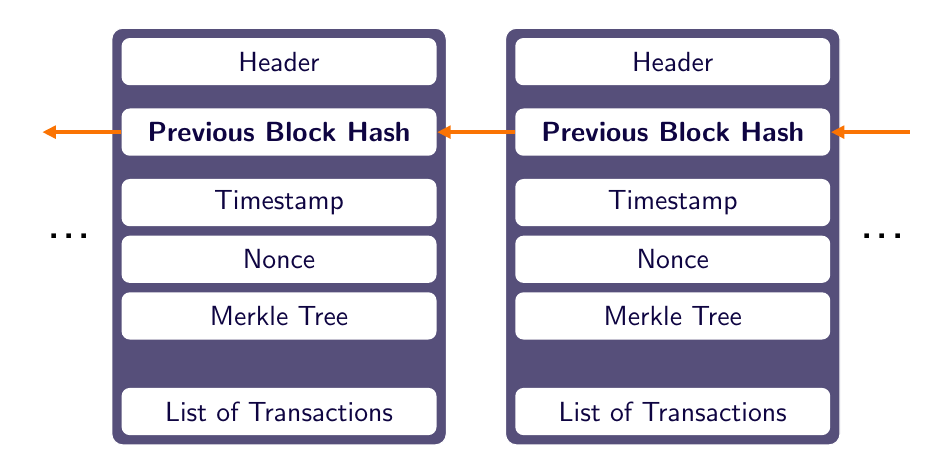
\begin{tikzpicture}[
        %Environment Cfg.
        font=\sffamily,
        >={Triangle[angle=50:3pt 2]},%from arrows.meta
        %Environment Styles.
        iBox/.style={
            rectangle,
            xscale= 1,
            % inner sep=0pt,
            minimum height=6mm,
            minimum width=40mm,
            rounded corners=3pt,
            % draw=Blue!50,  
            fill=white,   
            text=Blue
            % edge={Blue, ultra thick},
            % font=\sffamily\bfseries,
            % blur shadow,
            % rounded corners, 
            % draw={Orange!90, ultra thick}
        },
        eBox/.style={
            rectangle,
            rounded corners=4pt,
            draw=white,
            fill=Blue!70       
        },
    ]
    %Create repetitive objet with some variables like order name N, N+1 ...
    %\Block[hash block order][block order]{block-coordinate}
    \def\Block[#1][#2]#3{
        \begin{scope}[shift={(#3)}]
            \draw
            (0,0)
                node[iBox=3.5cm](HASH-#2){\textbf{Previous Block Hash}} %node[options](can be omitted){text_content}
                node[iBox=3.5cm, above right = 8pt and 0pt of HASH-#2.north west](VER)
                {Header}
                
                node[iBox, below = 8pt and 0pt of HASH-#2.south](TIM){Timestamp}
                node[iBox, below = 3pt and 0pt of TIM.south](NONC){Nonce}
                
                node[iBox=3.5cm, below = 3pt and 0pt of NONC.south](STE){ Merkle Tree} 
                
                node[iBox=3.5cm,below = 0.6cm of STE](LoT){ List of Transactions};
                \begin{scope}[on background layer] % from tikzlibrary backgrounds
                    \node[eBox,fit=(VER)(LoT),outer sep =5pt,](BK-#2){};
                \end{scope}
        \end{scope}
    }

    %Start drawing the thing.
    \Block[N-1][N]{0,0};
    \Block[N][N+1]{5,0};
    % \Block[N+1][N+2]{9.6,0};
    %Draw final details.
    \node[left=-5pt of BK-N,scale=2]{...};
    \node[right=-5pt of BK-N+1,scale=2]{...};
    \draw[->,very thick, Orange](HASH-N+1)--(HASH-N);
    % \draw[->,very thick, Orange](HASH-N+2)--(HASH-N+1);
    \draw[<-,very thick, Orange](HASH-N+1.east)--++(1cm,0);
    \draw[->,very thick, Orange](HASH-N.west)--++(-1cm,0);

    \end{tikzpicture}   
\end{document}